% Zusammenfassung und Ausblick
%

\chapter{Discussion}

\section{Circuit properties}


The generated full mouse brain circuit contains around 74 million neurons and 660 billion synapses.
From the neuron HDF5 file 12 parameters are used by the simulation.
It contains further parameters which are used for the connection generation and the visualization,
like coordinates. In total the neuron HDF5 file is of the size of around 9 GB.
The synapse HDF5 file only contains needed parameters for the simulation.
There are 5 synapse parameter per connection. This results in 15 TB of data.

So the generated circuit contains around 15 TB and is spitted in three HDF5 files (Neuron file, long range synapses file and short range synapses file). The interpolation which are added to the circuit generation introduces new errors, but allow
a first simulation of a full circuit model. Thus is allows to run and test is full pipeline from Allen Brain data to a NEST simulation. If there are more experiments available they can be included into
the circuit generation easily. The size of the circuit wont change. Thus no changes are needed anywhere else.


\begin{table}[ht!]
\begin{centering}
    \begin{tabular}{ | l | l | r | r | r |}
    \hline
    Identifier & ratio & neurons & synapses & total size \\ \hline \hline
    threehundredths & $0.3\%$ & $~2.5*10^5$ & $~2.2*10^9$ & $~26$ GB \\ \hline
    quater & $25\%$ & $~1.9*10^7$ & $~1.6*10^{11}$ & $~4$ TB \\ \hline
    full & $100\%$ & $~7.5*10^7$ & $~7.2*10^{11}$ & $~16$ TB \\ \hline
    \end{tabular}
    \caption{The circuits \emph{3hundredths}, \emph{1quater} and \emph{full} were created for testing and debugging on different scales.
All circuits were generated with identical parameters, only the input neuron file varies.}
\end{centering}
    \end{table}


\label{table:circuits}

Three different circuits (see Table \ref{table:circuits}) are generated: The full mouse brain circuit,
a smaller circuit, which contains 25 percent of the full mouse brain circuit and
1 300st of the full circuit. The percentage is related to the number of neurons inside
the circuit. Based on the neurons the connections are generated. In principle the
number of connections should be of the same proportion, but can deviate, because of 
discrete picking based on probabilities.


\begin{figure}[ht!]
\centering
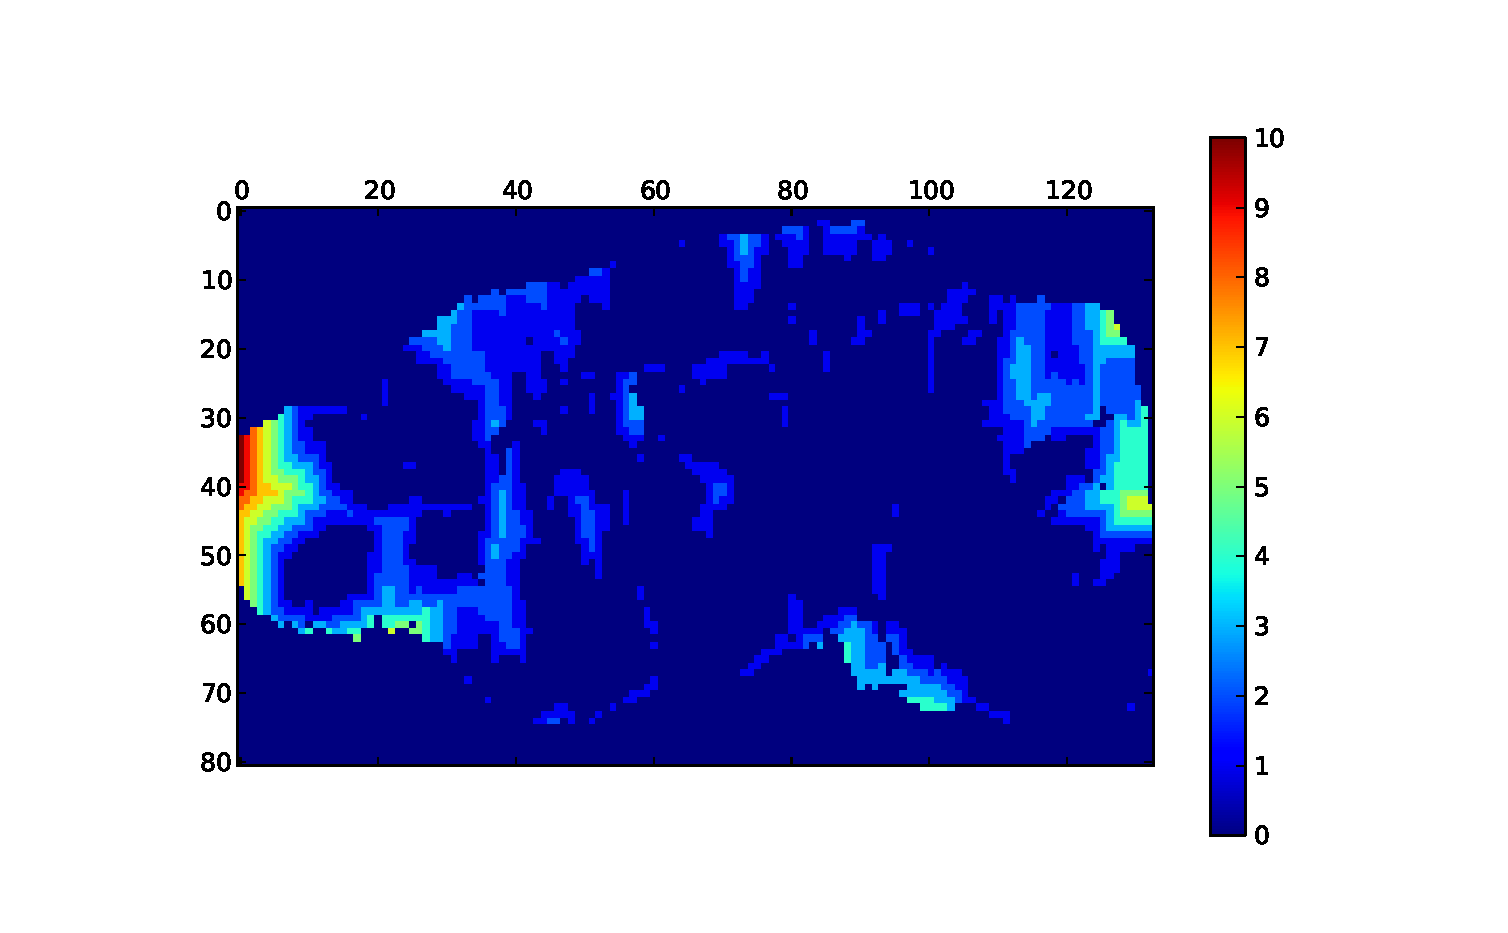
\includegraphics[scale=0.5]{pictures/distance_x_y_70.eps}
\caption{Plotted values from the nearest neighbor algorithm. You can see the distance to the next injected voxel.}
\label{interpolationdistance}
\end{figure}

\begin{figure}[ht!]
\centering
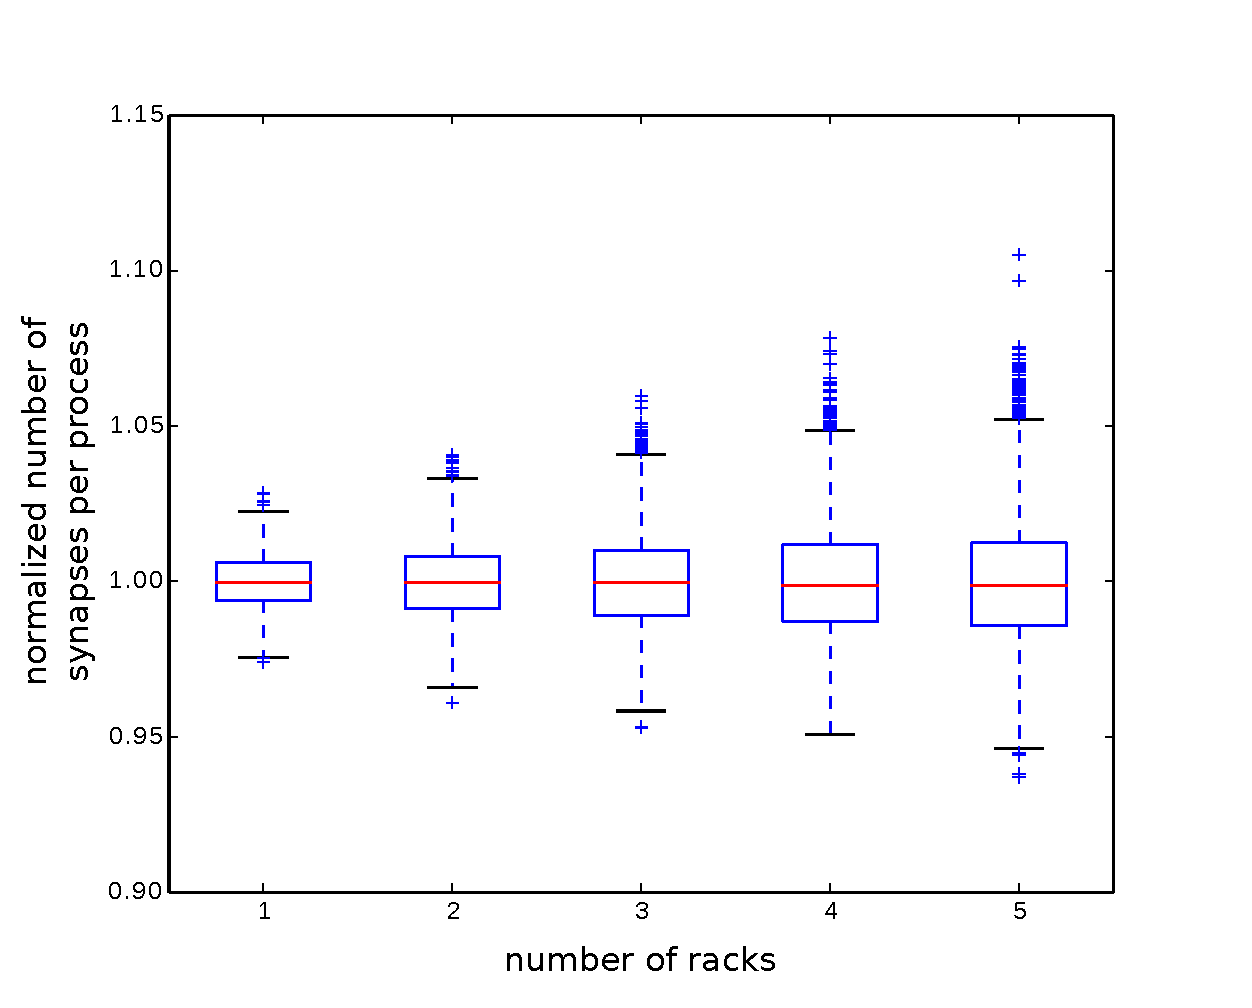
\includegraphics[scale=0.4]{pictures/full_circuit_rack_distribution.eps}
\caption{Estimated synapse imbalance of neuron distribution on processes.
It shows the distributions of relative sums (sum of number of synapses per process divided by mean of sums) of synapses per process (y-scale) on different scales (x-axis) }
\label{fullcircuitdist}
\end{figure}

The neurons are distributed equably on all processes based on equation \ref{eq:ProcessByNeuron}.
But the number of incoming synapses varies between the neurons.
Therefore a memory imbalance could occur between the processes.
To analyse the imbalance, an analysing script iterates over the \emph{syn} dataset and counts
the number of incoming synapses per neuron. Normalized results are plotted in box-plot diagrams 
in Figure \ref{fullcircuitdist}. An optimization for a specific simulation run is possible


\section{Data format usability}
The HDF5 data format for neuron parameters is used as given from the Neurorobotics team.
Because of its small size (9 GB) in comparison to the synapse dataset (15 TB) the performance improvement by changing
to a transposed data format can be neglected. Thus the usability of having different datasets and being able
to add new datasets can be kept. It also implies that the generation script does not have to be converted or no 
conversion scripts are needed.

\section{Performance}
Runtime measurements of the import module are performed on different scale.
Therefore IBM Blue Gene Q systems in Lugano and Juelich are used.

\subsection{Long range connections generation}
The sequential algorithm is optimized and parallelized. Moving the best injection per voxel search outside the main iteration
avoids unnecessary calculations and reduces the complexity of the main iteration. Further optimization are applied
to the linear acceptance rejection functionality, which picks the neurons in the projection area.
In the given sequential algorithm each neuron has its own probability.
But as given by the assignment all neurons in each voxel have the same value.

So at first a target voxel is picked and afterwards a neuron is selected from the chosen voxel.
This reduces the complexity of the picking from number of neurons in projection to number of voxels in projection.
For the full circuit this corresponds to a reduction of the order of 2.


\subsection{Short range connections generation}
The sequential algorithm could be ported directly to a parallel implementation without changing it.
Using a Master-Slave approach also reduced the complexity of the distribution of independent iterations.
The only issue is the writing of the file, because the number of created synapses is not know in the beginning.
Using a buffer or temporary files is necessary to return a non chunk based HDF5 file.
Because of the given resources (IBM Blue Gene Q) and the high parallel efficiency (see later section)
wirting all synapses to memory is feasible (already for a small number of nodes the created connections fit in memory).

\subsection{Import circuit}
Four parts of the synapse loading algorithm are instrumented to get wall clock timings.
\emph{Read}, \emph{Sort}, \emph{Alltoall} and \emph{Connect} are considered to be the mots time
consuming parts of the algorithm. The parts relate to figure \ref{Algparts}.
\emph{Def. Node} is negligible (It takes less than 1 percent computation time of an iteration and scales constant with the number of nodes.).
The following figures \ref{fig:implV03} give an overview of the measured wall-clock timings.
The timings are shown per node and iteration number. They give an idea how the timings are distributed.
The performance of the different parts can be compared and bottlenecks can be found.
%\begin{figure}[ht!]
%     \begin{center}
%        \subfigure[Load hdf5 files]{%
%            \label{fig:first}
%            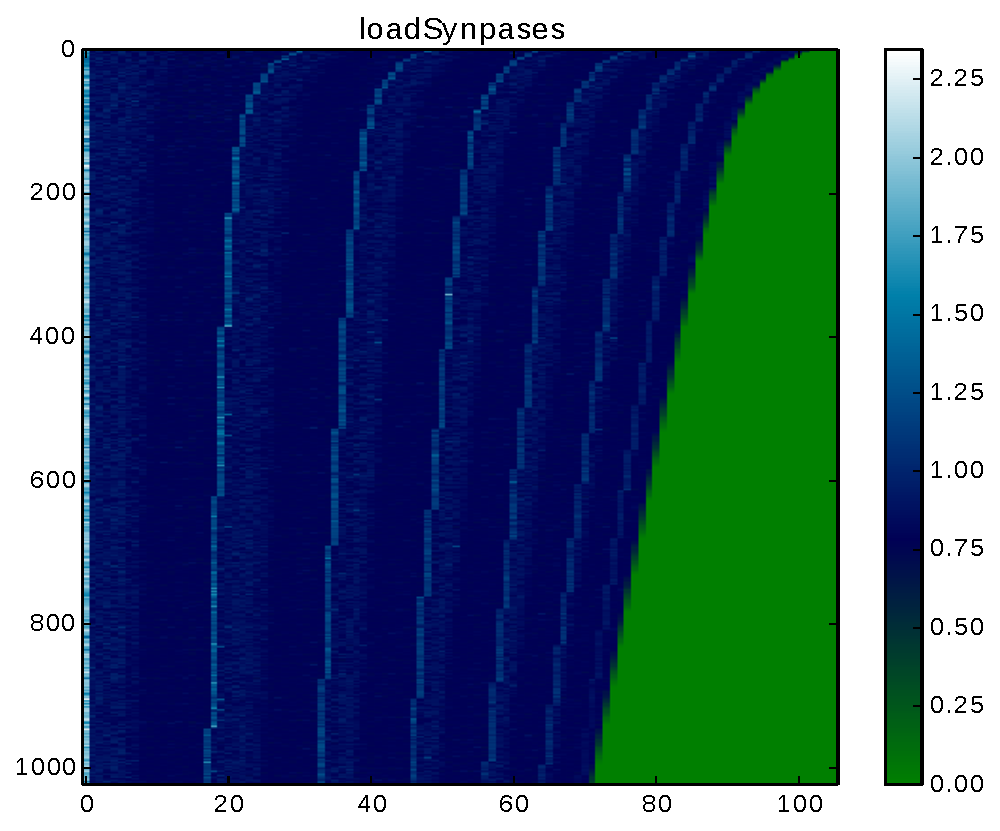
\includegraphics[width=0.45\textwidth]{pictures/V03_loadSynapses.eps}
%        }
%        \subfigure[Sort connection information data by target node]{%
%           \label{fig:second}
%           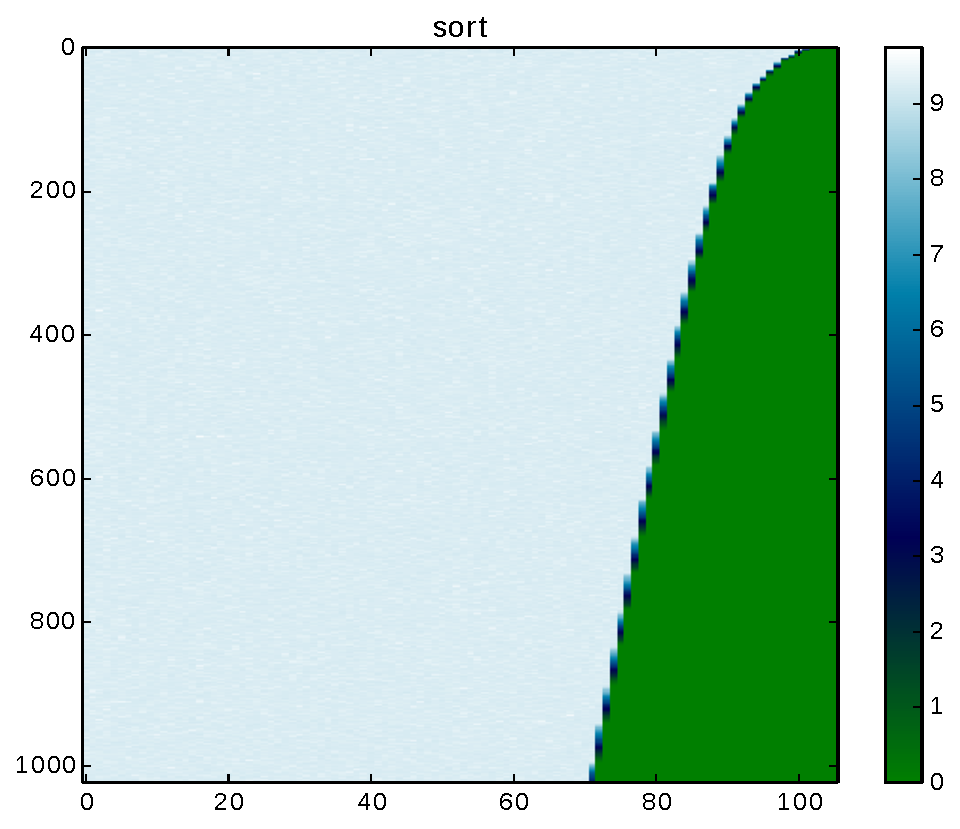
\includegraphics[width=0.45\textwidth]{pictures/V03_sort.eps}
%        }\\ %  ------- End of the first row ----------------------%
%        \subfigure[Send data to all target nodes using AlltoAllv]{%
%            \label{fig:third}
%            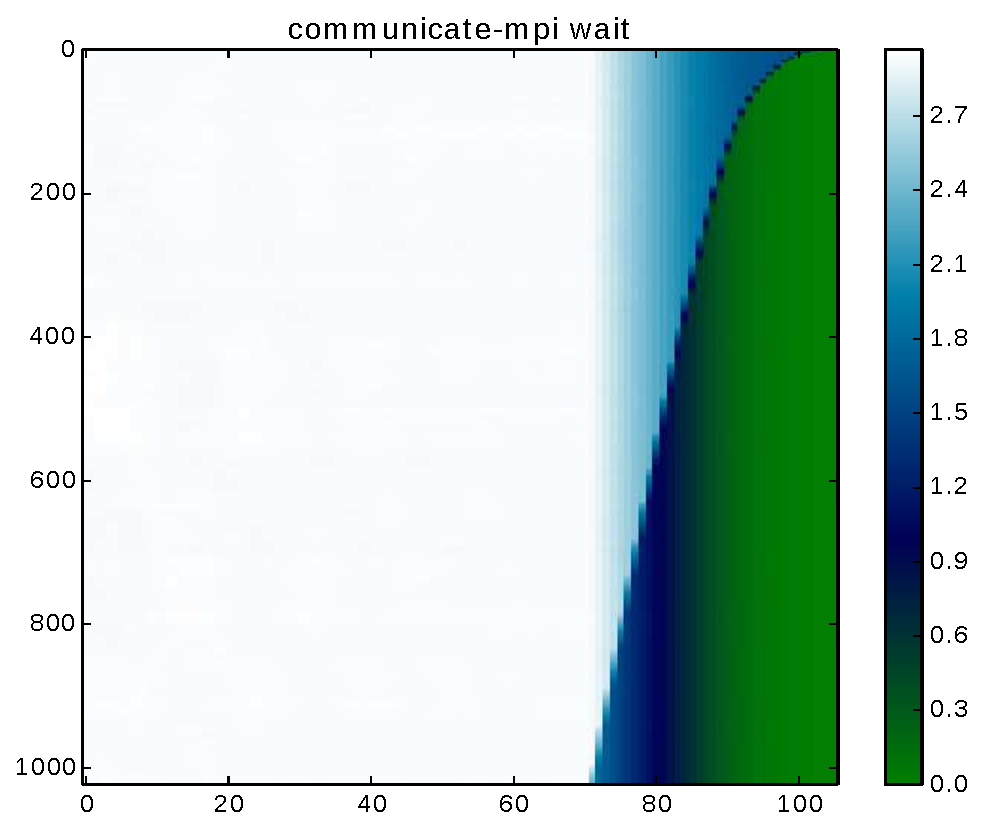
\includegraphics[width=0.45\textwidth]{pictures/V03_communicate.eps}
%        }
%        \subfigure[Connect function which calculated delay and calls NEST connect]{%
%            \label{fig:fourth}
%            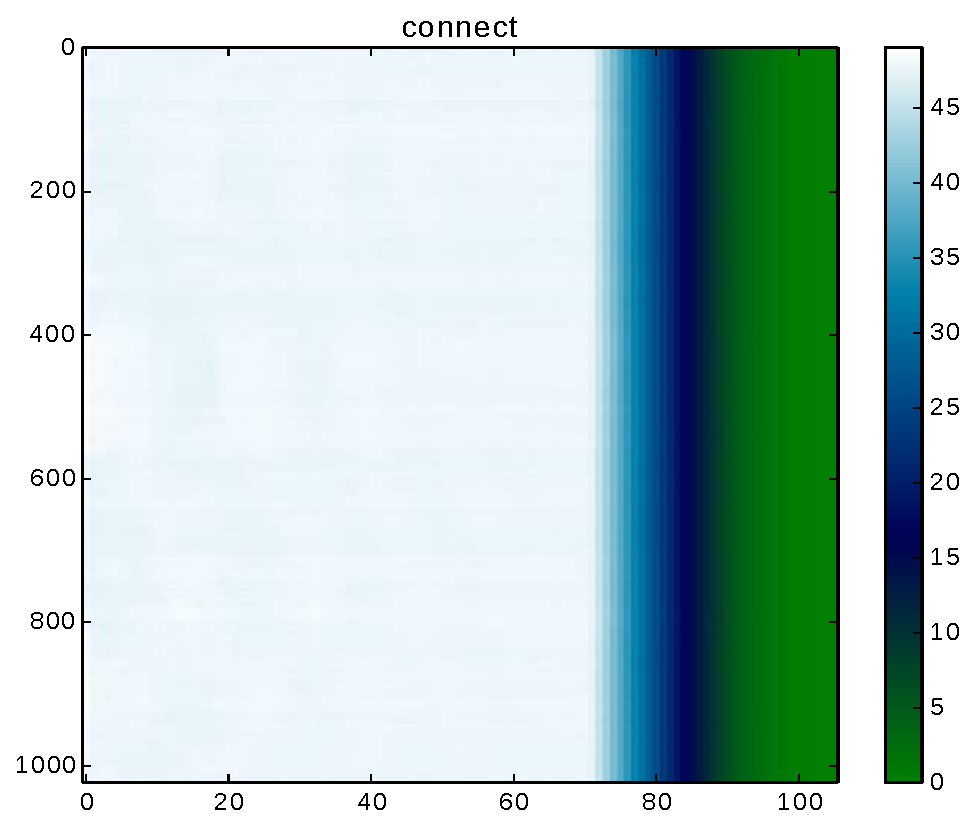
\includegraphics[width=0.45\textwidth]{pictures/V03_connect.eps}
%        }
%    \end{center}
%    \caption{%
%        The the plots show the the execution time for node per iteration.
%        The y-axes corresponds to the node id and the x-axes corresponds to the iteration number.
%        The color scale is in seconds.
%        In each iteration loadSynapses loads max $1e6$ synapses from hdf5 file.
%     }%
%   \label{fig:implV03}
%\end{figure}
One can see that \emph{Read} and \emph{Connect} are the critical parts.
For the interpretations of the plots one has to take into account that different parts of the algorithm
(\emph{Read} and \emph{Alltoall}) contain mpi collective operations and contain therefor mpi waits.
Thus the wall-clock timings do not satisfy the pure step functionality but also the imbalance from previous steps.
To analyse the impact, an experiment is performed which extends the implementation with \emph{MPI\_Barriers}
between the algorithm steps.
\newpage
\subsubsection{Read step}
The efficiency of the \emph{Read} step is bounded by the io bandwidth of the system.
Blue Brain IV has a theoretical bandwidth of $50$ GB/s per rack.

The amount of data read in \emph{Read} step depends on the number of synapse parameters $N_{params}$,
the number of read synapses per iteration $N_{blocksize}$ and the number of processes $N_{processes}$.
This results in measured bandwidth of:
\begin{equation}
b = sizeof(float) * N_{params} * \frac{N_{blocksize} * N_{processes}}{\Delta T}
\end{equation}
\subsubsection{Connect step}

Thread parallelization of the connect step allows to store the synapses efficiently in the NEST data structure.
The pure connect functionality of NEST is thread-safe. But creating and destroying SLI data objects is not and can result
in data-races. To overcome this limitation the creation and destroying of the objects is serialized. Before iterating over all synapses one SLI object is created and destroyed afterwards for each thread. A single connect function
call of the NEST api expects the synapse parameters stored in a SLI object. In each iteration the current
parameters are assigned to the values inside the already created SLI object. This SLI object is passed to the function call.
Thus a small overhead for the creation and destroying of the object is perceived.
\begin{figure}[ht!]
\centering
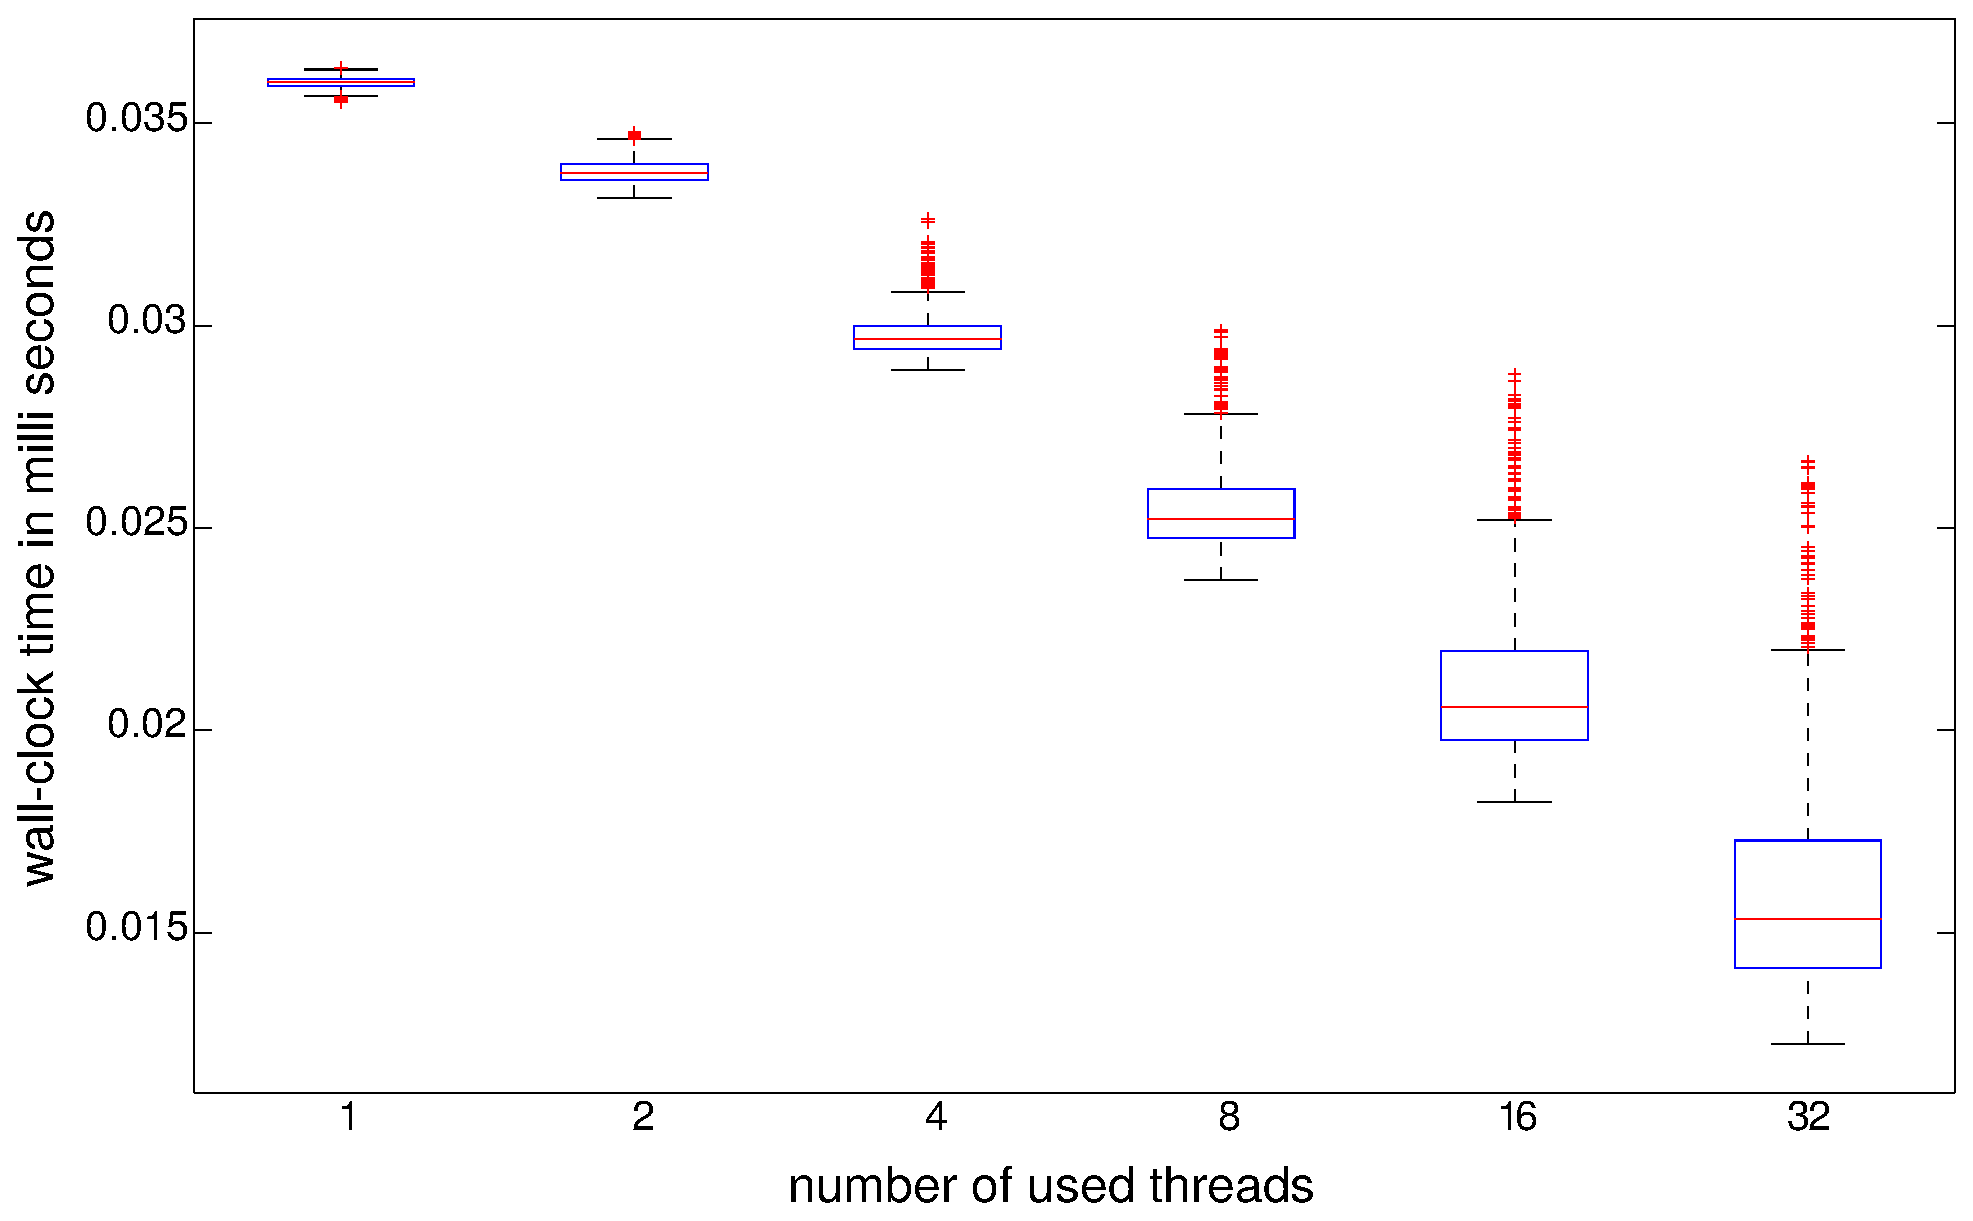
\includegraphics[scale=0.3]{pictures/boxplot_new_con_dt_1_300_edit.eps}
\caption{Comparison of mean of single connect duration across one iteration on one node.}
\label{boxplotnewcon}
\end{figure}
Because each thread iterates over all synapses, but only stores the connection if the target neuron is located on
the thread, the connection calls per thread varies.
As for nodes the neurons are distributed in the modules fashion on the threads for one node.
The distribution properties are the same. Thus there is a larger variation on a larger number of threads.
Figure \ref{boxplotnewcon} shows wall-clock time measurements for the connect step. The measurements are
extracted from the execution of the 1per300 circuit. It is executed on 128 nodes with varying number of
threads. The circuit plus fixed number of nodes specify the distribution of neurons per node.
The variations of the timings correlates with the distribution of synapses per node (figure \ref{fullcircuitdist}).
To look into detail, figure \ref{detailnewcon:second} shows the measured wall-clock time for each node
plotted over the maximum number of new connections per thread. It shows a strong correlation between the variable and
the duration. Thus the increasing variations of timings can be explained by the variations of synapses per thread.
The figure indicates two different timings per connection. There is an offset of regression between the pink
and the red dots. Pink an red dots represent all measurements with less than 40,000 and more than new synapses per
node respectively. Figure \ref{detailnewcon:first} shows the density of number of new synapses per node.
Less synapses results in a smaller vector size. There seems to be a loss of efficiency, which properly result from
the use of different cache levels. 

\begin{figure}[ht!]
     \begin{center}
        \subfigure[Histogram showing measured densities of number of new synapses per iteration step for one process.]{%
            \label{detailnewcon:first}
            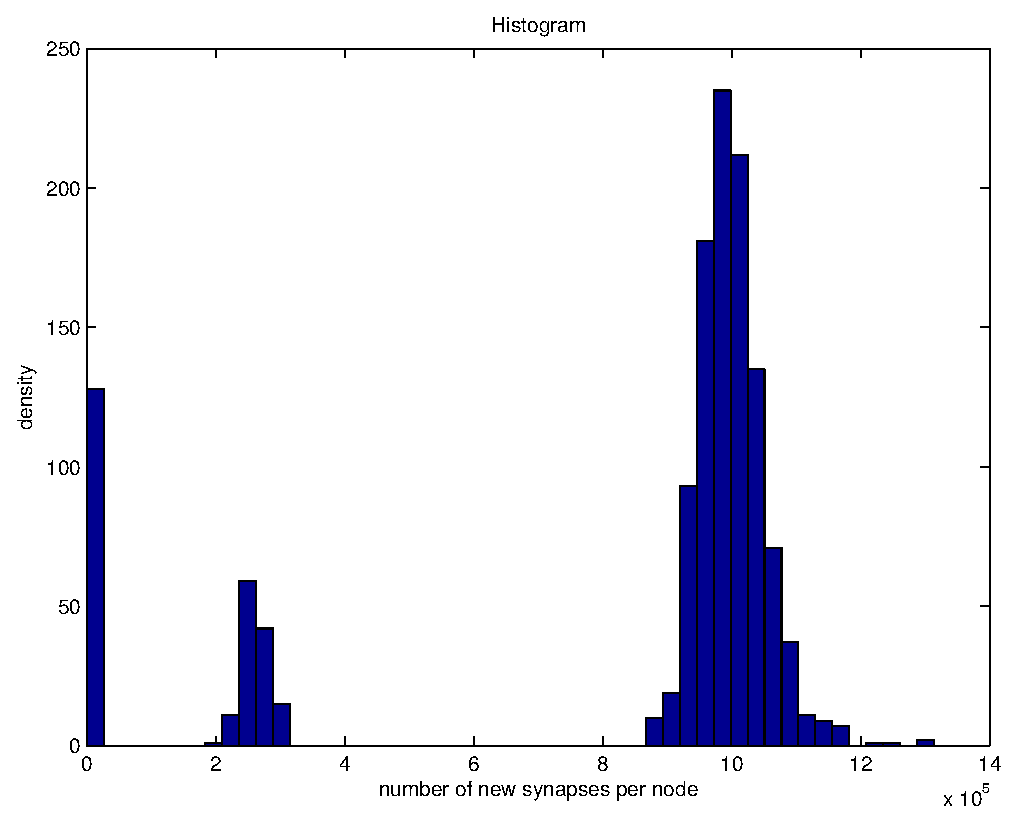
\includegraphics[scale=0.41]{pictures/histogram_new_const_1_300.eps}
        }
        \subfigure[Plotted wall-clock timings of \emph{connect} step over the number of new synapses for one thread
        			(Thread is part of process from Figure \ref{detailnewcon:first}. The new synapses are part of the new synapses from the process).
        			Pinks and red dotes relate to iterations, where the number of new synapses is smaller and bigger than $4*10^5$,
        			respectively (The values relate to the hills from Figure \ref{detailnewcon:first}). 
        			]{%
           \label{detailnewcon:second}
           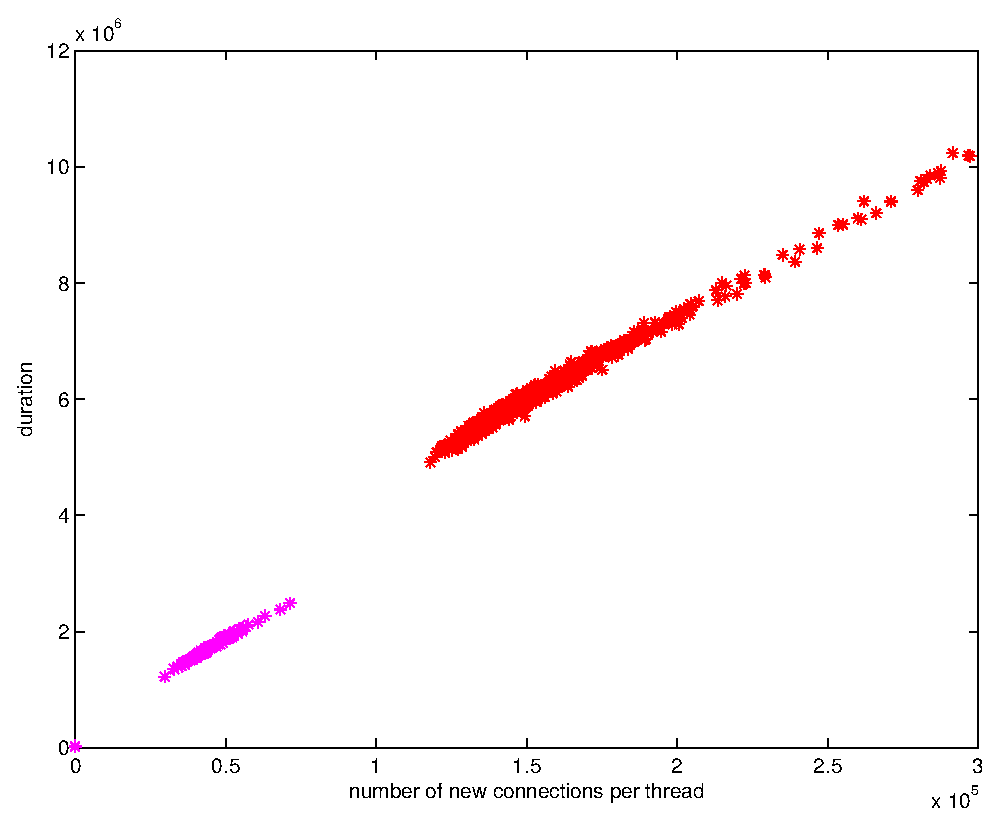
\includegraphics[scale=0.41]{pictures/t8_duration_per_con_1_300.eps}
		}
    \end{center}
    \caption{%
        The measurements are taken the same simulation run with the 1per300 circuit. It is run on the Blue Brain IV.
     }%
   \label{detailnewcon}
\end{figure}



\newpage
\section{Parallel Efficiency}

\subsection{Long range connections generation}
\subsection{Short range connections generation}
\subsection{Import circuit}

\begin{itemize}
      \item Tested in Lugano BGQ and Juelich BGQ
      \item Strong scaling
      \item Weak scaling
\end{itemize}

%\begin{figure}[!h] \centering
%\begin{tikzpicture}
%	\begin{axis}[title=AMBM CONNECT MODULE,
%		legend style={at={(0.5,-0.20)},
%		anchor=north,legend columns=-1},
%		xlabel=number of racks,
%		ylabel=Parallel efficiency (\% of linear scaling),
%		width=8.5cm
%		]
%
%	\addplot[color=blue,mark=*] coordinates {
%		(1,100)
%		(2,110)
%		(4,30)
%	};
%	\addplot[color=red,mark=*] coordinates {
%		(1,100)
%		(2,114)
%		(4,117)
%	};
%	\addplot[color=green,mark=*] coordinates {
%		(1,100)
%		(2,84)
%		(4,54)
%	};
%	\addplot[color=yellow,mark=*] coordinates {
%		(1,100)
%		(2,91)
%		(4,110)
%	};
%	\legend{io,sort,mpi,connect}
%	\end{axis}%
%\end{tikzpicture}%
%\begin{tikzpicture}
%	\begin{axis}[title=AMBM CONNECT MODULE,
%		legend style={at={(0.5,-0.20)},
%		anchor=north,legend columns=-1},
%		xlabel=number of racks,
%		ylabel=wall clock in seconds,
%		width=8.5cm
%		]
%
%	\addplot[color=blue,mark=*] coordinates {
%		(1,73)
%		(2,33)
%		(4,60)
%	};
%	\addplot[color=red,mark=*] coordinates {
%		(1,85)
%		(2,37)
%		(4,12)
%	};
%	\addplot[color=green,mark=*] coordinates {
%		(1,278)
%		(2,163)
%		(4,132)
%	};
%	\addplot[color=yellow,mark=*] coordinates {
%		(1,171)
%		(2,93)
%		(4,38)
%	};
%	\legend{io,sort,mpi,connect}
%	\end{axis}%
%\end{tikzpicture}%
%\end{figure}
%\begin{figure}[!h] \centering
%\begin{tikzpicture}
%	\begin{axis}[title=AMBM NEST RUN,legend style={at={(0.5,-0.20)}, anchor=north,legend columns=-1},
%		xlabel=number of racks,ylabel=Parallel efficiency (\% of linear scaling),width=8.5cm]
%
%	\addplot[color=blue,mark=*] coordinates {
%		(1,100)
%		(2,93)
%		(4,72)
%	};
%	\addplot[color=red,mark=*] coordinates {
%		(1,100)
%		(2,94)
%	};
%	\addplot[color=red,mark=o] coordinates {
%		(1,100)
%		(2,94)
%		(4,101)
%	};
%	\legend{mod,slisim, slisim estimated}
%	\end{axis}%
%\end{tikzpicture}%
%\begin{tikzpicture}
%	\begin{axis}[title=AMBM NEST RUN,legend style={at={(0.5,-0.20)}, anchor=north,legend columns=-1},
%		xlabel=number of racks,ylabel=wall clock in seconds,width=8.5cm]
%
%	\addplot[color=blue,mark=*] coordinates {
%		(1,640)
%		(2,344)
%		(4,220)
%	};
%	\addplot[color=red,mark=*] coordinates {
%		(1,1208)
%		(2,637)
%	};
%	\addplot[color=red,mark=o] coordinates {
%		(1,1208)
%		(2,637)
%		(4,299)
%	};
%	\legend{mod,slisim, slisim estimated}
%	\end{axis}%
%\end{tikzpicture}%
%\end{figure}

\section{Measured memory consumption}

\subsection{Long range connection generation}



\subsection{Short range connection generation}
\subsection{Load circuit}

\newpage
\section{Usability for Scientists}

\subsection{Manipulation of circuit}

\begin{itemize}
      \item control circuit generation / possibilities
      \item  manipulate circuit
\end{itemize}

\subsection{Import neurons}
\emph{H5NeuronCsX\_s\_s\_a\_s} expects 4 input parameters:
\begin{itemize}
      \item Name of the a subnet dataset (String).
The subset has to contain for each neuron an integer value.
The neurons are grouped together by this subnet value.

      \item A list of all datasets which values are interpreted as list of parameters.
      
      \item Name of the used neuron model
      
      \item path to the HDF5 file 
\end{itemize}
The function returns the neuron id of the first neuron it created.

\begin{lstlisting}[label=sliNeurons,caption=Calling the neuron import module via H5NeuronCsX\_s\_s\_a\_s SLI command ]
/neuronmodel /aeif_cond_exp def
/subnet (subnet) def
/neuronparams [(C_m) (Delta_T) (E_L) (V_reset) (V_th) (a) (b)] def
/filepath (circuit/ptneu_brain.h5) def
subnet neuronparams neuronmodel filepath H5NeuronCsX_s_s_a_s /offset Set
\end{lstlisting}



\begin{itemize}
      \item Sli command with parameters
      \item How can it be used
\end{itemize}

\subsection{Import synapses}
\emph{H5SynapseTll\_i\_s\_a\_s} expects 4 input parameters:
\begin{itemize}
      \item Offset of the neuron ids. Mostly it is equal to first neuron id returned by \emph{H5NeuronCsX\_s\_s\_a\_s}

      \item A list of all columns which values are interpreted as parameters.
      
      \item Name of the used synapse model
      
      \item path to the HDF5 file 
\end{itemize}
The function returns the neuron id of the first neuron it created.

\begin{lstlisting}[label=sliSynapses,caption=Example importing synapses]
/synmodel /tsodyks2_synapse def
/synparams [(delay) (weight) (U0) (TauRec) (TauFac)] def
/filepath (circuit/syn.h5) def
offset synparams synmodel filepath H5SynapseTll_i_s_a_s
\end{lstlisting}
\begin{itemize}
      \item How can it be used
\end{itemize}

\subsection{NEST simulation options}

Only one use-case (\ref{s}) of the mouse brain model is used in this thesis for performance evaluations.
Never the less more use-cases are realizable with the given implementations.
In general the neuron load module can be used equivalent to the neuron create function
and the synapses load module can be used equivalent to the neuron connect function.
Further a given circuit can be loaded and adapted (use offset or scaling factor for parameters).
Load neurons can be divided into subsets. The SLI functionality allow to access neuron sets
from the subnets. Thus the grouping performed with the subnet dataset is available for all SLI functions.
Stimulus generator and \emph{Spikedetector} or \emph{Multimeter} can be used to stimulate
and observe specific neurons respectively.
Furthermore SLI connect functions can be used to strengthening or weakening the connections between to
parts of the circuit.

\begin{itemize}
	  \item Test different stimuli
	  \item how to get results
\end{itemize}

\subsection{Analysis}
\begin{itemize}
	  \item Visualize spiking activity with Brion/Paraview
      \item Visualize spiking activity with ViSNEST
\end{itemize}